\documentclass[11pt]{article}

% XeTeX engine (tectonic): do NOT load inputenc; UTF-8 is native.
\usepackage[margin=1in]{geometry}
\usepackage{amsmath,amssymb}
\usepackage{booktabs}
\usepackage{array}
\usepackage{graphicx}
\usepackage{xcolor}
\usepackage{tikz}
\usetikzlibrary{arrows.meta,positioning,fit,backgrounds}
\usepackage{pgfplots}
\pgfplotsset{compat=1.18}
\usepackage[numbers,sort&compress]{natbib}
\usepackage[colorlinks=true,linkcolor=black,citecolor=blue,urlcolor=blue]{hyperref}
% let long URLs in the bibliography break anywhere (kills overfull bbl lines)
\usepackage{xurl}
\Urlmuskip=0mu plus 1mu\relax
\usepackage{titlesec}

\titleformat{\section}{\normalfont\large\bfseries}{\thesection}{0.6em}{}
\titleformat{\subsection}{\normalfont\normalsize\bfseries}{\thesubsection}{0.5em}{}
\setlength{\parskip}{0.35em}
\setlength{\parindent}{0pt}

% left-ragged fixed-width column: avoids underfull \hbox in narrow cited cells
\newcolumntype{L}[1]{>{\raggedright\arraybackslash}p{#1}}

\newcommand{\pat}[1]{\textsc{#1}}

% Title kept text-only (no \textbf / \\) so it extracts cleanly into
% plain-text metadata (digest/email/HTML).
\title{What Ships: A Practitioner's Catalogue of Applied AI Product
Patterns in Startups, 2024--2026}

\author{Yash Singh\\
\small IIIT Una}

\date{19 July 2026}

\begin{document}
\maketitle

\begin{abstract}
Between 2024 and 2026, applied AI product development went through a period of
convergent evolution: startups working largely independently kept arriving at
the same product shapes, the same orchestration architectures, and the same
pricing structures. The underlying constraints (probabilistic outputs,
context-window limits, per-token cost, and user trust) are the same
everywhere, and they admit only so many good answers. This paper names those
shapes. We synthesize public engineering writing,
framework documentation, vendor pricing pages, practitioner surveys, and
press-reported traction into a catalogue of twenty patterns organized in four
layers: \emph{interaction} (how users meet the model), \emph{orchestration}
(how model calls compose into systems), \emph{data and context} (what the model
is given to work with), and \emph{trust and economics} (how the system is made
dependable and paid for). For each pattern we state the problem it solves, the
startups shipping it, and the failure mode of skipping it. We pair the
catalogue with six recurring anti-patterns, short case vignettes of companies
whose public traction validates particular stacks, and a decision guide mapping
product requirements to pattern combinations. Our contribution is synthesis and
naming rather than new empirical results: the thesis is that applied AI has
quietly accumulated a reusable pattern language, and that most of the
difference between AI products that ship and AI demos that stall is disciplined
selection from this catalogue rather than novel research.
\end{abstract}

\section{Introduction}

The distance between a working model demo and a working AI product is now well
documented: practitioner surveys consistently rank response quality, cost, and
safety as the top blockers standing between agent prototypes and production
deployment \citep{langchain2024state}. Yet a
growing set of startups has crossed that distance repeatedly and at speed.
Cursor, Harvey, Sierra, Decagon, and the app-builder generation
(v0, Lovable, Bolt, Replit) ship continuously on top of the same handful of
frontier models available to everyone else. Whatever separates them from the stalled
majority is not model access.

We argue it is largely \emph{pattern selection}. When many teams converge on
the same solution shape under the same constraints, that shape is
worth naming, cataloguing, and teaching, which is precisely the premise of the
pattern-language tradition in architecture \citep{alexander1977pattern} and
software design \citep{gamma1995design}. Applied AI in mid-2026 has reached the
point where such a catalogue can be written down: the interaction idioms have
stabilized (inline copilots, artifact generation, background agents with review
gates), the orchestration playbook has been articulated by the model vendors
themselves \citep{anthropic2024agents, openai2025agentsguide}, context
engineering has displaced prompt engineering as the operative discipline
\citep{anthropic2025context, sourcegraph2026context}, and pricing has visibly
pivoted from seats toward work performed \citep{bvp2026pricing,
sierra2024outcomes}.

This paper makes four contributions:

\begin{enumerate}
  \item \textbf{A four-layer map} (Section~\ref{sec:layers}) that organizes
  applied AI product decisions into interaction, orchestration, data and
  context, and trust and economics.
  \item \textbf{A catalogue of twenty patterns}
  (Sections~\ref{sec:interaction}--\ref{sec:trust}), each with the problem it
  solves, exemplar products, and the cost of skipping it.
  \item \textbf{Six anti-patterns} (Section~\ref{sec:antipatterns}) that
  recur in practitioner accounts of stalled AI products.
  \item \textbf{Case vignettes and a decision guide}
  (Sections~\ref{sec:vignettes}--\ref{sec:decision}) connecting the catalogue
  to companies whose press-reported traction suggests the patterns compose
  profitably.
\end{enumerate}

Like its predecessors in the patterns tradition, this paper reports practice
rather than inventing it. Every pattern here is observable in shipping
practice under the inclusion test of Section~\ref{sec:method}; none is
speculative.

\section{Related work}
\label{sec:related}

The form of this paper borrows deliberately from the pattern-language
tradition. Alexander et al.\ showed that recurring solution shapes in a
design discipline can be mined from practice, named, and composed
\citep{alexander1977pattern}, and Gamma et al.\ carried the method into
software \citep{gamma1995design}. We apply the same recurrence test to a much
younger discipline; the price of that youth is the drift limitation discussed
in Section~\ref{sec:limitations}.

The academic literature approaches the same terrain from the research side.
Surveys of LLM-based agents organize systems by cognitive component: planning,
memory, and tool use \citep{wang2024agentsurvey}; the retrieval-augmented
generation line runs from the original formulation \citep{lewis2020rag}
through comprehensive surveys of its variants \citep{gao2023ragsurvey};
and Kapoor et al.\ critique how agent research is evaluated, arguing that
benchmark-maximizing agents diverge from agents that are useful in deployment
\citep{kapoor2024agentsmatter}. This catalogue is complementary to that body
of work: our unit of analysis is the shipping product rather than the
published system, and our layers follow the order in which product teams make
decisions rather than the internal architecture of an agent.

Closest to our aim are the vendor playbooks: Anthropic's guidance on building
effective agents \citep{anthropic2024agents} and OpenAI's practical guide
\citep{openai2025agentsguide} are prescriptive and practice-derived, and both
are widely read. They concentrate on the orchestration layer, however. The
catalogue here spans interaction, data, and economics as well, imposes an
explicit three-product inclusion test, and pairs the patterns with the
anti-patterns teams report when they stall.

\section{Scope and method}
\label{sec:method}

\textbf{Sources.} We draw on four kinds of public evidence: (i) engineering
writing by model vendors and infrastructure companies
\citep{anthropic2024agents, anthropic2025multiagent, openai2025agentsguide,
bornstein2023emerging, mlflow2026production, arize2026patterns}; (ii) framework and protocol
documentation, particularly around tool integration \citep{anthropic2024mcp};
(iii) practitioner surveys and investor field reports
\citep{langchain2024state, menlo2025enterprise, bvp2026pricing}; and (iv)
product surfaces themselves: pricing pages, changelogs, and press-reported
traction \citep{intercom2026fin, sierra2024outcomes, forbes2026cursor}.

\textbf{Inclusion criterion.} A pattern enters the catalogue only if it is
observable in at least three independent shipping products from different
companies. ``Shipping'' means generally available and paid for, not
demonstrated at a conference. For infrastructure- and data-layer patterns
whose deployments are mostly internal (workflow substrates, gateways, eval
harnesses, retrieval pipelines, fine-tuning programs), the three-product test
was applied against public engineering writing, and Table~\ref{tab:catalogue}
sometimes names the practice rather than three logos. Although the catalogue
is aimed at startups, we cite incumbent and frontier-lab products (GitHub
Copilot, Notion AI, Deep Research) where they are the clearest instance of a
pattern; the unit of the catalogue is the pattern, not the company. We also
scope out modality-specific interaction (voice and real-time agents, which
several of our exemplar companies ship) and several near-universal
implementation techniques that sit below the product-pattern grain: streaming
and partial-result UX, cache-aware prompt layout, input-side prompt-injection
defense, and first-run onboarding for blank-canvas products. Each deserves
treatment of its own.

\subsection{Limitations}
\label{sec:limitations}

Four biases are unavoidable. \emph{Survivorship}: we see
the patterns of companies that succeeded enough to write about them.
\emph{Disclosure}: revenue and traction figures are press-reported, not
audited; we cite them as directional evidence only. \emph{Drift}: this field
re-tools quickly, and the catalogue is a snapshot dated mid-2026.
\emph{Diffusion}: not all convergence is independent; the vendor playbooks
\citep{anthropic2024agents, openai2025agentsguide} are widely read, so we
cannot always distinguish teams rediscovering a shape under shared
constraints from teams adopting a published one. We treat both as evidence
that the shape survives production use, which is the property the catalogue
certifies, while noting that it weakens any inference of inevitability. We
mitigate the first bias by including anti-patterns sourced from practitioner
writing and survey-reported failure modes, the second by labeling every
traction figure as press-reported, and the third by preferring patterns with
at least eighteen months of visible use.

\section{A four-layer map}
\label{sec:layers}

Product decisions in applied AI cluster into four layers
(Figure~\ref{fig:stack}). The layers are ordered by proximity to the user, and
in practice they are also ordered by how early the decision gets made: teams
choose an interaction shape first, discover the orchestration it requires,
then discover the data machinery that orchestration needs, and confront trust
and economics last, usually later than they should.

\begin{figure}[tbp]
\centering
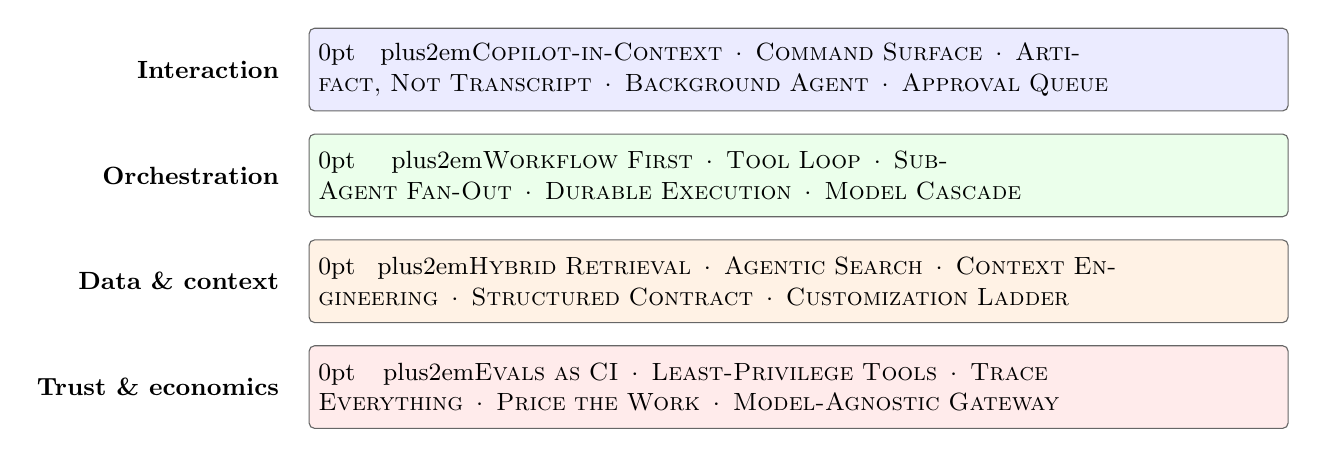
\begin{tikzpicture}[
  layerbox/.style={draw=black!60, rounded corners=2pt, minimum height=1.05cm,
    text width=12.2cm, align=center,
    font=\small\hyphenpenalty=10000\exhyphenpenalty=10000},
  lab/.style={font=\small\bfseries, anchor=east}
]
  \node[layerbox, fill=blue!8]  (l1) {\pat{Copilot-in-Context} \,\(\cdot\)\, \pat{Command Surface} \,\(\cdot\)\, \pat{Artifact, Not Transcript} \,\(\cdot\)\, \pat{Background Agent} \,\(\cdot\)\, \pat{Approval Queue}};
  \node[layerbox, fill=green!8, below=0.28cm of l1] (l2) {\pat{Workflow First} \,\(\cdot\)\, \pat{Tool Loop} \,\(\cdot\)\, \pat{Sub-Agent Fan-Out} \,\(\cdot\)\, \pat{Durable Execution} \,\(\cdot\)\, \pat{Model Cascade}};
  \node[layerbox, fill=orange!10, below=0.28cm of l2] (l3) {\pat{Hybrid Retrieval} \,\(\cdot\)\, \pat{Agentic Search} \,\(\cdot\)\, \pat{Context Engineering} \,\(\cdot\)\, \pat{Structured Contract} \,\(\cdot\)\, \pat{Customization Ladder}};
  \node[layerbox, fill=red!8, below=0.28cm of l3] (l4) {\pat{Evals as CI} \,\(\cdot\)\, \pat{Least-Privilege Tools} \,\(\cdot\)\, \pat{Trace Everything} \,\(\cdot\)\, \pat{Price the Work} \,\(\cdot\)\, \pat{Model-Agnostic Gateway}};
  \node[lab, left=0.25cm of l1] {Interaction};
  \node[lab, left=0.25cm of l2] {Orchestration};
  \node[lab, left=0.25cm of l3] {Data \& context};
  \node[lab, left=0.25cm of l4] {Trust \& economics};
\end{tikzpicture}
\caption{The four-layer map with the twenty catalogued patterns. Upper layers
are visible to users; lower layers are visible in the margin structure and the
incident log.}
\label{fig:stack}
\end{figure}

Table~\ref{tab:catalogue} summarizes the full catalogue; the next four
sections walk through each layer.

\begin{table}[tbp]
\centering
\small
\begin{tabular}{@{}l L{3.3cm} L{5.4cm} L{4.3cm}@{}}
\toprule
\# & Pattern & What it buys you & Exemplars \\
\midrule
I1 & \pat{Copilot-in-Context} & Zero-friction help inside the existing workflow & Cursor Tab, GitHub Copilot, Notion AI \\
I2 & \pat{Command Surface} & Natural language as an accelerator over structured UI & Linear, Superhuman, Raycast AI \\
I3 & \pat{Artifact, Not Transcript} & Output is an editable object, not chat prose & v0, Lovable, Bolt, Claude Artifacts \\
I4 & \pat{Background Agent} & Minutes-long work moved off the interaction path & Devin, Claude Code, Deep Research \\
I5 & \pat{Approval Queue} & Delegation without giving up the final say & Fin drafts, Sierra handoffs, Clay outreach \\
\midrule
O1 & \pat{Workflow First} & Predictability where the task shape is known & Support triage, document pipelines \\
O2 & \pat{Tool Loop} & Open-ended tasks via model-directed tool calls & Coding agents, computer use \\
O3 & \pat{Sub-Agent Fan-Out} & Parallelism plus context isolation & Anthropic research system, OpenAI and Gemini Deep Research \\
O4 & \pat{Durable Execution} & Agents that survive restarts and retries & Temporal/Inngest-backed agent products \\
O5 & \pat{Model Cascade} & Most traffic served below frontier-model cost & Routing layers in support and search \\
\midrule
D1 & \pat{Hybrid Retrieval} & Recall from lexical + vector + reranking & Glean, Perplexity, enterprise RAG \\
D2 & \pat{Agentic Search} & Retrieval as an iterated tool, not one shot & Deep Research (OpenAI, Gemini), Cursor codebase QA \\
D3 & \pat{Context Engineering} & Deliberate budget for what the model sees & Claude Code, ChatGPT memory, Letta \\
D4 & \pat{Structured Contract} & Model output as a typed API, not prose & Extraction products, generative UI \\
D5 & \pat{Customization Ladder} & Prompt \(\to\) RAG \(\to\) fine-tune, in that order & Vertical AI (Harvey), high-volume tasks \\
\midrule
T1 & \pat{Evals as CI} & Regressions caught before users see them & Golden sets + LLM-judge in CI \\
T2 & \pat{Least-Privilege Tools} & Bounded blast radius for agent actions & Sandboxes, allowlists, spend caps \\
T3 & \pat{Trace Everything} & Debuggable multi-step failures & LangSmith, Arize, MLflow tracing \\
T4 & \pat{Price the Work} & Margin aligned with value delivered & Fin \$0.99/resolution, Sierra outcomes \\
T5 & \pat{Model-Agnostic Gateway} & Model swaps in days, not quarters & Gateway layers, provider abstraction \\
\bottomrule
\end{tabular}
\caption{The pattern catalogue at a glance.}
\label{tab:catalogue}
\end{table}

\section{Interaction patterns}
\label{sec:interaction}

\subsection{I1: Copilot-in-Context}

\textbf{Problem.} Users will not leave their working surface to consult a
model, and copy-pasting context into a chat window loses the state that makes
suggestions relevant.

\textbf{Pattern.} Embed generation \emph{inside} the existing artifact at the
point of attention: inline code completion, inline rewrite, cell-level
spreadsheet fills. The model sees the surrounding document state; the user
accepts with a keystroke. Cursor's Tab completion is the canonical example,
and its press-reported multi-billion-dollar revenue run rate
\citep{forbes2026cursor} is consistent with low-friction, high-frequency
invocation being where individual willingness to pay concentrates.
Latency budgets here are hundreds of milliseconds, which forces small or
distilled models and aggressive caching, connecting this pattern directly to
\pat{Model Cascade} (O5).

\textbf{Skip it and:} your AI feature lives in a side panel nobody opens.

\subsection{I2: Command Surface}

\textbf{Problem.} Structured products accumulate hundreds of operations that
users cannot remember how to reach.

\textbf{Pattern.} A natural-language command layer over the product's existing
actions: ``move everything assigned to me due this week to the next cycle.''
The model's job is intent parsing and parameter filling against a typed action
schema (see \pat{Structured Contract}, D4), not free generation. Linear,
Superhuman, and Raycast all ship this shape. It is the safest first AI feature
for an established SaaS product because the action set is already audited:
the model chooses among known operations rather than inventing new ones.

\textbf{Skip it and:} you build an open-ended chatbot that can discuss the
product but not operate it, which users try once.

\subsection{I3: Artifact, Not Transcript}

\textbf{Problem.} Chat transcripts are a poor container for work products.
Users need to edit, version, share, and deploy what the model makes.

\textbf{Pattern.} The unit of output is a live artifact (an app, a document, a
deck, a diagram) rendered beside the conversation and directly editable.
Vercel's v0, Lovable, Bolt, and Claude's Artifacts all converged on the same
split-pane shape within roughly a year of each other. The conversation becomes the
\emph{editing instrument}; the artifact is the product. Karpathy's framing of
natural language as the new programming interface \citep{karpathy2025software}
is this pattern generalized: the prompt is source, the artifact is the build.

\textbf{Skip it and:} users screenshot your chat output into their real tools,
and the value accrues to those tools.

\subsection{I4: Background Agent}

\textbf{Problem.} Real tasks (a research report, a pull request, a data
migration) take minutes to hours, and no user will watch a spinner for that
long.

\textbf{Pattern.} Move the agent off the interaction path: the user files a
task, the agent works asynchronously with \pat{Durable Execution} (O4), and
returns a reviewable result such as a diff, a draft, or a cited report.
Devin, Claude Code's cloud sessions, OpenAI's Deep Research, and the
current generation of coding and research agents all share this shape. The
critical design choice is the \emph{return artifact}: it must be reviewable in
minutes even though it took the agent an hour, which is why diffs and
cited reports dominate.

\textbf{Skip it and:} you either cap task ambition at chat latency, or ship
long-running work with no checkpoint, no cancellation, and no review surface.

\subsection{I5: Approval Queue}

\textbf{Problem.} Organizations want delegation without surrendering
accountability, and regulators are moving toward human-oversight requirements
for consequential automated actions (e.g., the EU AI Act's Article~14
\citep{euact2024}).

\textbf{Pattern.} The agent produces \emph{proposed} actions (a support reply,
an outbound email, a journal entry) that accumulate in a queue where humans
approve, edit, or reject; approval rates are tracked and gate progressive
autonomy. Support products (Fin, Sierra, Decagon) run this pattern for
escalations; GTM products like Clay run it for outreach. The queue doubles as
a labeling pipeline: every human edit is training and eval data
(\pat{Evals as CI}, T1).

\textbf{Skip it and:} the first bad autonomous action becomes a churn event or
a headline.

\section{Orchestration patterns}
\label{sec:orch}

\subsection{O1: Workflow First}

\textbf{Problem.} Teams reach for autonomous agents when the task has a known,
decomposable shape, and inherit non-determinism they did not need.

\textbf{Pattern.} When the steps are knowable in advance, hard-code them:
prompt chaining (fixed task decompositions of the kind chain-of-thought
prompting made visible \citep{wei2022cot}), routing, parallelization,
orchestrator-workers, and
evaluator-optimizer loops, in Anthropic's articulation
\citep{anthropic2024agents}, echoed by OpenAI's guidance to start with the
simplest composition that works \citep{openai2025agentsguide}. A workflow's
control flow lives in code, so it is testable, traceable, and cheap. The
practitioner heuristic that survives contact with production is: \emph{use
workflows for predictability, agents for flexibility, and workflows until
proven otherwise}.

\textbf{Skip it and:} you debug an agent's planning on tasks that never needed
planning.

\subsection{O2: Tool Loop}

\textbf{Problem.} Some tasks genuinely cannot be decomposed in advance:
debugging, open-ended research, multi-system operations.

\textbf{Pattern.} The reason-act loop \citep{yao2023react}, now internalized
as native tool calling: the model chooses tools, observes results, and
iterates until a stop condition, with self-correction along the way
\citep{shinn2023reflexion, madaan2023selfrefine}; see
\citet{wang2024agentsurvey} for the academic lineage. What changed between 2023
and 2026 is not the loop but its harness: production tool loops now run
inside budget caps, step limits, and \pat{Least-Privilege Tools} (T2), and
their traces feed \pat{Evals as CI} (T1). Tool-augmented modeling was
demonstrated early \citep{schick2023toolformer}; the surprise is how much of
the engineering lives outside the model. The integration surface has
meanwhile standardized: the Model Context Protocol, introduced in late 2024
\citep{anthropic2024mcp} and since adopted by the other major providers, has
become a de facto standard for exposing tools to models, letting one tool
loop reach thousands of external systems without bespoke adapters.

\textbf{Skip it and:} you lose nothing if your tasks are decomposable, and
everything if they are not.

\subsection{O3: Sub-Agent Fan-Out}

\textbf{Problem.} A single context window cannot hold a large task, and long
contexts degrade attention over their middle \citep{liu2024lost}.

\textbf{Pattern.} An orchestrator decomposes the task and spawns parallel
sub-agents, each with a clean, scoped context; results are synthesized.
Anthropic's public account of its research system reports substantial quality
gains from exactly this isolation-plus-parallelism structure
\citep{anthropic2025multiagent}. The pattern's tax is coordination:
sub-agents cannot see each other's discoveries unless the orchestrator routes
them, so it fits tasks that decompose cleanly (research, review, migration
sweeps) better than tightly coupled edits. Cognition's engineering guidance
argues against multi-agent designs for exactly the coupled case
\citep{cognition2025dontbuild}; that is the boundary of this pattern, not a
refutation of it.

\textbf{Skip it and:} large tasks either overflow the window or degrade
quietly as the context fills.

\subsection{O4: Durable Execution}

\textbf{Problem.} A thirty-minute agent run \emph{will} encounter a rate
limit, a deploy, or a crash, and users will not accept losing twenty-nine
minutes of work.

\textbf{Pattern.} Treat agent steps as checkpointed, replayable workflow
activities: persist state after every tool call, make tools idempotent, and
resume from the journal rather than restarting. Startups increasingly run
agent loops on durable-execution substrates (Temporal, Inngest, or
homegrown queues) so that retries, timeouts, and human-approval pauses
(\pat{Approval Queue}, I5) are first-class. The substrate vendors' own
guidance frames durable execution as the foundation for any agent that
outlives a request cycle \citep{temporal2025durable, inngest2026durable}.

\textbf{Skip it and:} your agent's reliability is the product of every
dependency's uptime, and that product rounds to zero over long runs.

\subsection{O5: Model Cascade}

\textbf{Problem.} Frontier-model pricing on every call destroys gross margin,
but small models alone cap quality.

\textbf{Pattern.} Route by difficulty: a cheap model (or a cache hit) handles
the easy majority, escalating to larger models only on low confidence,
following the cascade logic formalized in FrugalGPT \citep{chen2023frugalgpt}.
Production deployments layer semantic caching in front, then distilled or
small open models, then a frontier model, then (for some products) a human,
with each tier absorbing most of what reaches it (Figure~\ref{fig:cascade}).
The economics compress to one expression: with per-call cost $c_i$ at tier
$i$ and absorption rate $h_i$ (the fraction of traffic reaching tier $i$ that
stops there), expected cost per query over $n$ tiers is
\begin{equation}
\mathbb{E}[c] \;=\; \sum_{i=1}^{n} c_i \prod_{j=1}^{i-1}\bigl(1-h_j\bigr),
\label{eq:cascade}
\end{equation}
so the cheap tiers' absorption rates, not the frontier model's list price,
dominate unit cost. Inline copilots (I1) are the extreme case: their latency
budget alone forces the cascade. Margin pressure across the category is well
documented \citep{bvp2026pricing}.

\textbf{Skip it and:} you discover at scale that your unit economics require
charging more than users will pay.

\begin{figure}[tbp]
\centering
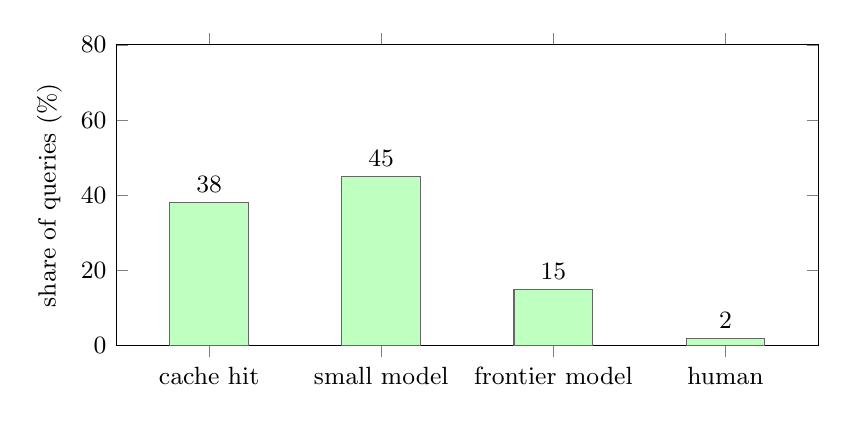
\begin{tikzpicture}
\begin{axis}[
  ybar, bar width=1.0cm,
  width=10.5cm, height=5.4cm,
  ymin=0, ymax=80,
  ylabel={\small share of queries (\%)},
  symbolic x coords={cache hit, small model, frontier model, human},
  xtick=data, x tick label style={font=\small},
  ytick={0,20,40,60,80}, y tick label style={font=\small},
  nodes near coords, every node near coord/.append style={font=\small},
  enlarge x limits=0.18,
]
\addplot[fill=green!25, draw=black!60] coordinates
  {(cache hit,38) (small model,45) (frontier model,15) (human,2)};
\end{axis}
\end{tikzpicture}
\caption{An \emph{illustrative} model cascade for a support-style workload
(bar values are notional, not measured): the cheap tiers together absorb the
large majority of traffic, so frontier-model spend applies to a small
residual. Real mixes vary by product; the shape recurs across them.}
\label{fig:cascade}
\end{figure}

\section{Data and context patterns}
\label{sec:data}

\subsection{D1: Hybrid Retrieval}

\textbf{Problem.} Pure vector search misses exact identifiers and rare terms;
pure lexical search misses paraphrase; either alone caps answer quality.

\textbf{Pattern.} Retrieval-augmented generation \citep{lewis2020rag} in its
matured production form \citep{gao2023ragsurvey}: lexical and vector retrieval
run together, a reranker orders the union, and metadata filters scope the
corpus. The standard fusion step is reciprocal rank fusion
\citep{cormack2009rrf}: a document $d$ ranked by retrievers $R$ scores
\begin{equation}
s(d) \;=\; \sum_{r \in R} \frac{1}{k + \mathrm{rank}_r(d)},
\label{eq:rrf}
\end{equation}
with $k \approx 60$ in common practice, cheap enough to run on every query. Enterprise search (Glean), answer engines (Perplexity), and virtually
every serious internal RAG deployment run this shape. A recurring
practitioner report of 2024--2025 was that retrieval quality, not model
choice, dominated answer quality for knowledge products
\citep{langchain2024state, menlo2025enterprise}.

\textbf{Skip it and:} your model fluently summarizes the wrong documents.

\subsection{D2: Agentic Search}

\textbf{Problem.} One-shot retrieval cannot answer questions that require
following leads: multi-hop questions, codebase questions, market research.

\textbf{Pattern.} Make retrieval a \emph{tool inside a loop} (O2): the model
searches, reads, reformulates, and searches again, accumulating evidence
before answering. Deep-research products and coding assistants' codebase
question-answering both replaced single-shot RAG with iterated search between
2024 and 2026. The cost is latency and tokens, which is why shipping products
pair it with \pat{Background Agent} (I4) rather than chat.

\textbf{Skip it and:} multi-hop questions get confident answers assembled from
the first page of results.

\subsection{D3: Context Engineering}

\textbf{Problem.} The context window is the binding resource, attention
degrades over long contexts \citep{liu2024lost}, and naive accumulation of
history, tool output, and retrieved text fills it with noise.

\textbf{Pattern.} Budget and curate everything the model sees on every call:
system state, retrieved evidence, tool results, and memory. In practice this
means compaction (rewriting older turns into summaries), tool-output
truncation with keep-or-drop rules, tiered memory with explicit
recall (the MemGPT lineage \citep{packer2023memgpt}), and per-call context
budgets \citep{anthropic2025context, sourcegraph2026context}. By 2026 this
discipline, not prompt wording, is what determines agent reliability; vendor
engineering guidance is explicit that context curation is the
highest-leverage lever for long-running agents.

\textbf{Skip it and:} your agent gets measurably dumber as the session gets
longer, and nobody can say why.

\subsection{D4: Structured Contract}

\textbf{Problem.} Downstream code cannot consume prose, and parsing free text
is a bug factory.

\textbf{Pattern.} Constrain output to a schema (JSON schema, function
signatures, typed DSLs) and treat the model as a typed API. This is the
load-bearing pattern beneath \pat{Command Surface} (I2), generative UI,
extraction products, and most B2B AI: the schema is simultaneously the
interface contract, the validation gate, and the eval target (exact-match
scoring against fields is cheap and objective, easing the evaluator-trust
problem of judging prose \citep{zheng2023judge}).

\textbf{Skip it and:} you maintain a regex museum between the model and your
database.

\subsection{D5: Customization Ladder}

\textbf{Problem.} Teams jump to fine-tuning for problems that prompting or
retrieval solve in a day, acquiring MLOps burden and a stale model.

\textbf{Pattern.} Climb in order: prompt engineering with few-shot examples
first; retrieval (D1) when the knowledge is the gap; fine-tuning only when
format, style, or latency at volume demand it, typically distilling a
frontier model's behavior on a narrow task into a small model that slots into
a cascade (O5). Vertical leaders like Harvey combine frontier models with
domain workflow and data rather than betting on bespoke base models; the
high-volume, narrow-task tier (classification, extraction, routing) is where
fine-tuned small models earn their keep.

\textbf{Skip it and:} you spend a quarter fine-tuning your way to what a
better retrieval pipeline would have delivered in a sprint.

\section{Trust and economics patterns}
\label{sec:trust}

\subsection{T1: Evals as CI}

\textbf{Problem.} Probabilistic systems regress silently: a prompt tweak,
model upgrade, or retrieval change shifts behavior with no compiler error.

\textbf{Pattern.} A golden dataset of real cases, scored on every change and
gating deploys exactly like tests: exact-match where outputs are structured
(D4), LLM-as-judge with periodic human calibration where they are prose
\citep{zheng2023judge}, and downstream task metrics where possible
\citep{kapoor2024agentsmatter}. Production guides treat systematic evaluation
as a first-class engineering discipline for agent teams
\citep{mlflow2026production}; survey data confirm quality is the
top adoption blocker \citep{langchain2024state}. The approval queue (I5) and
trace store (T3) feed the dataset continuously.

\textbf{Skip it and:} every deploy is a bet, and you find regressions via
churn.

\subsection{T2: Least-Privilege Tools}

\textbf{Problem.} An agent with broad credentials turns a model mistake or a
prompt injection into a production incident.

\textbf{Pattern.} Scope every tool to the minimum: allowlisted actions,
sandboxed execution, read-only defaults, spend and rate caps, and
human approval (I5) for irreversible operations. Vendor guidance formalizes
this as guardrails around both inputs and actions \citep{openai2025agentsguide},
and coding agents ship sandboxes by default. The tool schema becomes a
security boundary, reviewed like one.

\textbf{Skip it and:} your agent's first confidently wrong action writes to
production.

\subsection{T3: Trace Everything}

\textbf{Problem.} A five-step agent failure is invisible in request logs; the
error is distributed across model calls, tool results, and context state.

\textbf{Pattern.} Capture the full tree (prompts, tool calls, outputs, tokens,
latency, cost) for every run, as spans, and make it queryable. The tracing
substrate (LangSmith, Arize, MLflow, and homegrown equivalents) is what makes
agent debugging, cost accounting per feature, and eval-set mining
(T1) possible at all \citep{arize2026patterns, mlflow2026production}.

\textbf{Skip it and:} ``the agent did something weird yesterday'' is a bug
report you cannot act on.

\subsection{T4: Price the Work}

\textbf{Problem.} Seat-based pricing breaks twice for AI products: marginal
cost per use is nonzero (heavy users destroy margin), and the product's value
is the work performed, not the humans logged in; an agent that replaces labor
has no seat to price.

\textbf{Pattern.} Charge in units of work or outcome: per resolution
(Intercom's Fin at \$0.99 per resolved conversation \citep{intercom2026fin}),
outcome-based contracts (Sierra \citep{sierra2024outcomes}), usage-metered
credits (the app builders), or hybrid base-plus-usage, which investor field
data show displacing seat-only pricing, with category gross margins already
well below classic SaaS \citep{bvp2026pricing}. T4 and O5 are two sides of
one inequality: charging price $p$ per resolution at resolution rate $q$ is
viable only while
\begin{equation}
q\,p \;>\; \mathbb{E}[c],
\label{eq:unit}
\end{equation}
with $\mathbb{E}[c]$ the per-attempt serving cost of
Equation~\ref{eq:cascade}; outcome pricing is what makes the cascade a
requirement rather than an optimization. Two consequences follow: billing infrastructure
becomes product infrastructure (metering, attribution, dispute handling), and
the eval suite (T1) becomes a revenue system, because you only get paid for
resolutions you can verifiably count.

\textbf{Skip it and:} either customers subsidize your heavy users, or your
gross margin does.

\subsection{T5: Model-Agnostic Gateway}

\textbf{Problem.} Model rankings shuffle every few months, and a hard
dependency on one provider converts each release cycle into a migration.

\textbf{Pattern.} All model calls go through one internal gateway that owns
provider adapters, fallbacks, caching, routing (O5), and per-feature cost
attribution (T3). Prompts and evals (T1) are versioned per model, so
adopting a newly released model is an eval run plus a config change shipped
in days, not a migration project; this is what lets startups ride the
frontier rather than be disrupted by it.

\textbf{Skip it and:} you are one deprecation notice away from an unplanned
quarter of migration work.

\section{Anti-patterns}
\label{sec:antipatterns}

The catalogue's negative space is as consistent as its positive space.
Table~\ref{tab:anti} lists the six failures that recur in practitioner
writing and survey-reported failure modes \citep{langchain2024state,
menlo2025enterprise, kapoor2024agentsmatter, anthropic2024agents}.

\begin{table}[tbp]
\centering
\small
\begin{tabular}{@{}L{3.4cm} L{5.2cm} L{4.9cm}@{}}
\toprule
Anti-pattern & Symptom & Remedy \\
\midrule
Thin wrapper & Product is a prompt in front of an API; churn tracks the base model's improvements & Own workflow, data, and distribution; climb the layers (Fig.~\ref{fig:stack}) \\
Chat for everything & A text box replaces designed UX; users must invent their own prompts & I1/I2/I3: meet users inside their artifact \\
Agent maximalism & Autonomous agent deployed on decomposable tasks; nondeterminism with no payoff & O1: workflow until proven otherwise \citep{anthropic2024agents} \\
Demo-driven development & Impressive happy path, no eval set, quality regressions on every change & T1 before scale; measure the boring cases \citep{kapoor2024agentsmatter} \\
Premature fine-tuning & Months on a bespoke model that retrieval or prompting matches & D5: climb the ladder in order \\
Below-cost pricing & Flat pricing meets power users; negative gross margin at exactly the moment of product-market fit & T4 + O5: meter the work, cascade the cost \citep{bvp2026pricing} \\
\bottomrule
\end{tabular}
\caption{Recurring anti-patterns and their catalogue remedies.}
\label{tab:anti}
\end{table}

Two of these deserve a sentence more. \emph{Agent maximalism} is the most
expensive because it is the most seductive: the demo is genuinely better, and
the production behavior is genuinely worse, a gap that only an eval suite
(T1) makes visible before customers do \citep{kapoor2024agentsmatter}.
\emph{Thin wrapper} is the most misdiagnosed: wrappers fail not because
wrapping is bad but because the wrapper owns no layer of Figure~\ref{fig:stack}
below the first; the companies dismissed as wrappers that thrived (Perplexity,
Cursor) own retrieval, context, evals, and distribution.

\section{Case vignettes}
\label{sec:vignettes}

Traction figures below are press- or company-reported (cited per claim),
offered as directional evidence that these pattern stacks compose into businesses, not as
audited financials.

\textbf{Cursor} (AI coding). Pattern stack: I1 as the wedge (Tab
completions), I4 layered later (background agents), O5 forced by
completion latency, D3 for repository context, T5 to ride successive frontier
models. Press reports place its annualized revenue at \$2B in March 2026 and
\$4B by June 2026 \citep{techcrunch2026cursor, forbes2026cursor}; that growth
spans Tab and the agent modes, though the aggregate figure cannot be
attributed between them.

\textbf{Harvey} (legal). Pattern stack: D1/D5 (domain retrieval over
authorities and work product), O1 workflows shaped to legal deliverables, I5
review surfaces fitting professional accountability, T2 for privilege
boundaries. A March 2026 raise at an \$11B valuation, with a company-reported
100{,}000-plus lawyers across 1{,}300 organizations and a majority of the
AmLaw~100 as customers \citep{harvey2026raise}, supports the vertical thesis: the moat is
workflow depth and professional trust.

\textbf{Sierra} (customer service agents). Pattern stack: O1 routing with O2
escalation, I5 human handoffs, T1 evals tied to resolution counting, and
T4 as strategy, outcome-based pricing per resolution
\citep{sierra2024outcomes}. Press reports of \$100M ARR within two years
\citep{techcrunch2025sierraarr}, \$150M by mid-2026 \citep{cnbc2026sierra},
and a May 2026 raise at a \$15B+ valuation \citep{techcrunch2026sierra}
suggest that outcome pricing has not constrained enterprise adoption.

\textbf{Decagon} (support automation) runs the adjacent stack (I5, O1, T1,
usage-metered T4) and reached a press-reported \$4.5B valuation in February
2026, triple its prior round \citep{forbes2026decagon}. A valuation reflects
investor expectation rather than delivered work, so we weight this vignette
below the revenue-based ones; it still suggests the stack, not any single
company's execution, is the repeated element.

\textbf{The app builders} (v0, Lovable, Bolt, Replit). Pattern stack: I3 as
identity (the artifact is a deployed app), D4 underneath (generation targets
component and config schemas), credit-metered T4, T5 across models. Lovable's
climb to \$100M ARR within eight months of launch and Replit's to \$150M
annualized within a year \citep{techcrunch2025lovable, techcrunch2025replit}
track the maturation of I3 from demo to default.

\section{A decision guide}
\label{sec:decision}

Figure~\ref{fig:decision} compresses the orchestration choice;
Table~\ref{tab:decision} maps common product requirements onto pattern
stacks. Both
encode the same bias the vendor playbooks state outright
\citep{anthropic2024agents, openai2025agentsguide}: take the simplest
composition that meets the requirement, and add autonomy only when the task
shape is genuinely unknown.

\begin{figure}[tbp]
\centering
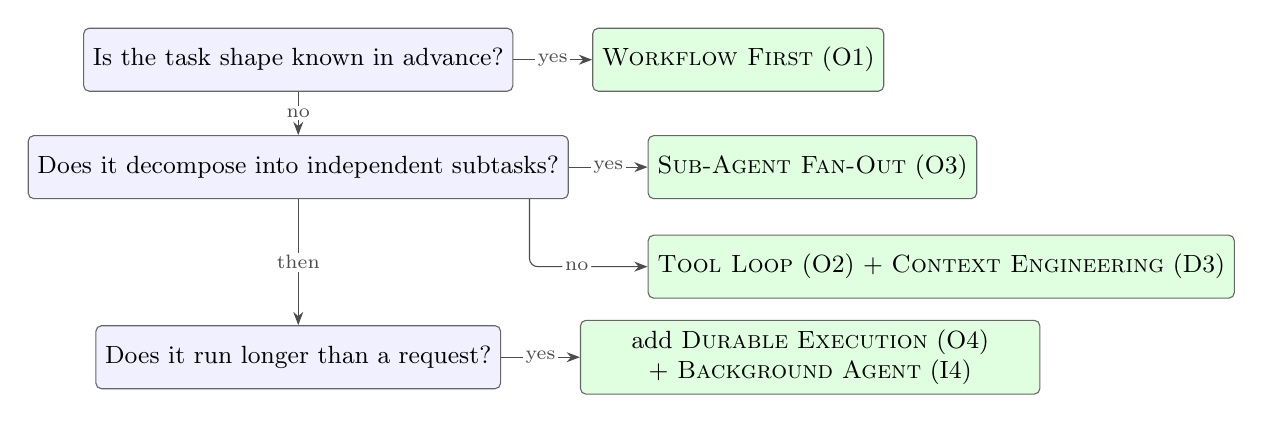
\begin{tikzpicture}[
  q/.style={draw=black!60, rounded corners=2pt, fill=blue!6, align=center,
    font=\small, minimum height=0.8cm},
  a/.style={draw=black!60, rounded corners=2pt, fill=green!12, align=center,
    font=\small, minimum height=0.8cm},
  e/.style={-{Stealth}, black!70},
  lbl/.style={font=\scriptsize, fill=white, inner sep=1pt}
]
  \node[q] (q1) {Is the task shape known in advance?};
  \node[a, right=1.0cm of q1] (a1) {\pat{Workflow First} (O1)};
  \node[q, below=0.55cm of q1] (q2) {Does it decompose into independent subtasks?};
  \node[a, right=1.0cm of q2] (a2) {\pat{Sub-Agent Fan-Out} (O3)};
  \node[a, below right=0.45cm and 0cm of a2.south west, anchor=north west]
    (a3) {\pat{Tool Loop} (O2) + \pat{Context Engineering} (D3)};
  \node[q, below=1.6cm of q2] (q3) {Does it run longer than a request?};
  \node[a, right=1.0cm of q3, text width=5.6cm] (a4) {add \pat{Durable Execution} (O4) + \pat{Background Agent} (I4)};
  \draw[e] (q1) -- node[lbl]{yes} (a1);
  \draw[e] (q1) -- node[lbl]{no} (q2);
  \draw[e] (q2) -- node[lbl]{yes} (a2);
  \draw[e, rounded corners=3pt] ([xshift=-5mm]q2.south east) |- node[lbl, pos=0.7]{no} (a3.west);
  \draw[e] (q2) -- node[lbl]{then} (q3);
  \draw[e] (q3) -- node[lbl]{yes} (a4);
\end{tikzpicture}
\caption{The orchestration decision. The first two questions choose a base
pattern; the third applies to whichever base was chosen (the edge is drawn
from the open-ended branch only to keep the figure compact) and overlays O4
and I4. Every path also gets T1 and T3; any path with side effects gets T2
and usually I5.}
\label{fig:decision}
\end{figure}

\begin{table}[tbp]
\centering
\small
\begin{tabular}{@{}L{4.6cm} L{8.9cm}@{}}
\toprule
Product requirement & Minimal pattern stack \\
\midrule
AI feature inside an existing SaaS & I2 + D4 + T1; add I1 if the product has an editing surface \\
Knowledge answers over a corpus & D1 + T1 + O5; add D2 when questions are multi-hop \\
Automate a back-office process & O1 + I5 + T1--T3; agents (O2) only for the exception path \\
Autonomous work product (code, research) & I4 + O2/O3 + O4 + D3 + T2 \\
High-volume narrow task (extract, classify, route) & D4 + D5 + O5; eval by exact match \\
Sell the outcome, not the software & everything above, plus T4 with metering you can defend in a billing dispute \\
\bottomrule
\end{tabular}
\caption{Requirements to pattern stacks. Every stack implicitly includes T3
(you cannot run what you cannot see) and T5 (you will change models).}
\label{tab:decision}
\end{table}

\section{Discussion and open problems}

The catalogue also exposes what practice has \emph{not} solved.

\textbf{Evaluator trust.} T1 increasingly leans on model judges
\citep{zheng2023judge} whose failure modes correlate with the systems they
judge; agent benchmarks remain easy to overfit and expensive to make
realistic \citep{kapoor2024agentsmatter}. Outcome pricing (T4) raises the
stakes: when the eval counts revenue, adversarial pressure on the eval is
guaranteed.

\textbf{Attribution for outcome pricing.} ``Per resolution'' works when a
conversation closes; it is unresolved for agents whose work is one input among
many (marketing, research, code that ships weeks later). Until attribution
matures, hybrid metering remains the honest default \citep{bvp2026pricing}.

\textbf{Trust UX for delegation.} I5 does not scale to agents proposing
hundreds of actions per day; nobody has shipped a convincing answer to
\emph{graduated} autonomy, where trust earned on one task class transfers
legibly to another.

\textbf{Margin structure under falling token prices.} Cascades (O5) and
falling frontier prices improve unit economics, but capability expectations
rise in lockstep, keeping spend per task roughly constant; whether AI-native
gross margins converge to SaaS norms or settle permanently lower
\citep{bvp2026pricing} will shape which patterns remain affordable.

\textbf{Defensibility.} The catalogue is public and the patterns are
imitable. The durable moats visible in the vignettes (workflow depth,
proprietary eval data, distribution) predate AI; whether pattern execution
alone compounds into defensibility is the category's open bet.

\section{Conclusion}

The applied AI products that ship in 2026 are not built from secret
techniques. They are built from a small, nameable catalogue of patterns that
teams keep arriving at, partly by independent rediscovery and partly by
adopting published playbooks, because the constraints (probabilistic outputs,
bounded context, per-token cost, human trust) admit only so many good
answers. We have named twenty of them, organized them into four layers, paired
them with the six failures teams repeat, and grounded them in the public
traction of companies whose stacks we can read from the outside. The practical
claim is modest and testable: for most AI product decisions in a startup
today, the right move already has a name in this catalogue, and the expensive
mistakes come from skipping a layer, not from missing research. Pattern
languages end with an invitation rather than a proof, and so does this one:
the catalogue is a snapshot of mid-2026, and it will be revised by the next
capability jump, most likely first at the interaction layer, where each jump
has rewritten what users meet.

% ragged-right bibliography: URL-heavy entries otherwise leave underfull lines
\begingroup
\raggedright
\bibliographystyle{plainnat}
\bibliography{refs}
\endgroup

\end{document}
